\documentclass[../Head/Main.tex]{subfiles}
\begin{document}
\subsection{Environment}
The two-wheeled robot should navigate around in the environment called “bigworld” shown on figure {\color{red} xx}. To do so more effectively, we have chosen to divide the world into 14 rooms and each of these rooms has been given a room number. This division is illustrated on figure {\color{red} yy} using a gray scale, where each room has been given a specific gray tone color.
\begin{figure}[H]
	\centering
	\begin{subfigure}[b]{0.49\textwidth}
		\centering
		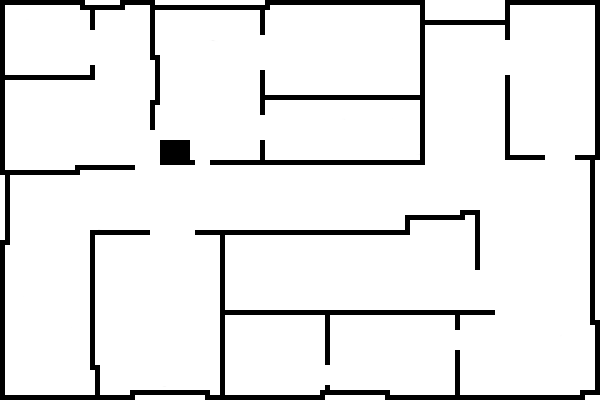
\includegraphics[width=\textwidth]{map_medium_white}
		\caption{Illustration of the world "bigworld"}
	\end{subfigure}
	\hfill	
	\begin{subfigure}[b]{0.49\textwidth}
		\centering
		%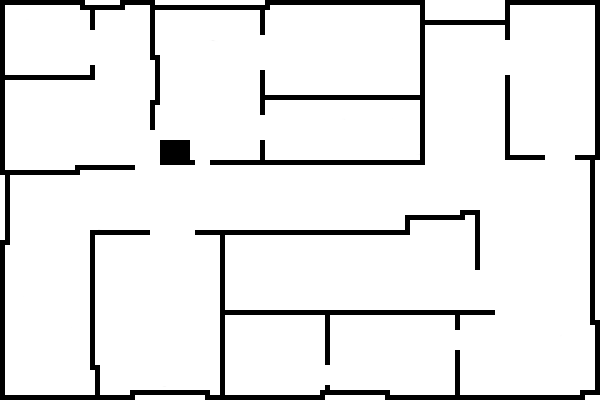
\includegraphics[width=\textwidth]{map_medium_white}
		%\subfile{../Figures/Bigworld_room_division}
		\begin{tikzpicture}
		\node[anchor=south west, inner sep=0] (image) at (0,0) {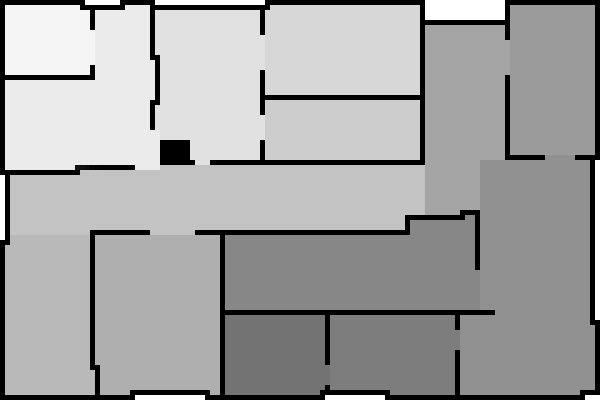
\includegraphics[width=\textwidth]{map_medium}};
		\node[align=center, black, font={\small}] at (0.7,5) {Room 1};
		\node[align=center, black, font={\small}] at (1.2,3.9) {Room 2};
		\node[align=center, black, font={\small}] at (2.9,4.5) {Room 3};
		\node[align=center, black, font={\small}] at (4.75,4.9) {Room 4};
		\node[align=center, black, font={\large\bfseries}] at (7.25,5.75) {Room 5};
		%\node[align=center, black, font={\large\bfseries}] at (5,4.25) {Room 6};
		%\node[align=center, black, font={\large\bfseries}] at (1,2) {Room 7};
		%\node[align=center, black, font={\large\bfseries}] at (3.3,2) {Room 8};
		%\node[align=center, black, font={\large\bfseries}] at (9.9,6.25) {Room 9};
		%\node[align=center, black, font={\large\bfseries}] at (11.75,6.75) {Room 10};
		%\node[align=center, black, font={\large\bfseries}] at (11.5,2.5) {Room 11};
		%\node[align=center, black, font={\large\bfseries}] at (7.25,2.75) {Room 12};
		%\node[align=center, black, font={\large\bfseries}] at (8.25,1) {Room 13};
		%\node[align=center, black, font={\large\bfseries}] at (5.8,1) {Room 14};
		\end{tikzpicture}		
		\caption{"bigworld" divided into 14 rooms}
	\end{subfigure}
\end{figure}

\end{document}